\documentclass{article}
\usepackage{amsmath}
\usepackage{amssymb}
\usepackage{graphicx}
\usepackage{hyperref}
\usepackage[version=4]{mhchem}

\title{Example 4}
\date{}

\begin{document}
\maketitle

(Phillips Academy Prize Exam) Bases \(A B\) and \(D C\) of a trapezoid \(A B C D\) are perpendicular to \(B C\) at \(B\) and \(C\) respectively. From \(P\), the midpoint of side \(A D\), lines are drawn to \(B\) and \(C\). Prove: \(P B=P C\).

Solution:
\begin{center}
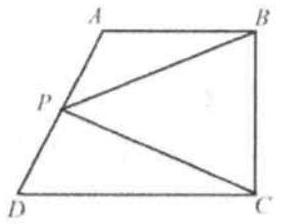
\includegraphics[width=\textwidth]{images/problem_image_1.jpg}
\end{center}

Given: Trapezoid \(A B C D\) with \(A B \perp B C, D C \perp B C\), and \(P\) is the midpoint of \(A D\). Let \(T\) be the midpoint of \(B C\). Since \(P T\) is the median of trapezoid \(A B C D\), then \(P T / / A B\), making \(P T\) the perpendicular bisector of \(B C\). Thus \(P B=P C\) because points on a perpendicular bisector are equidistance from the endpoints of a segment.\\
\centering
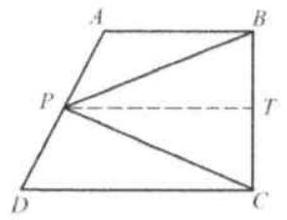
\includegraphics[width=\textwidth]{images/reasoning_image_1.jpg}


\end{document}
